% =========================================================================
% APÊNDICE: RESULTADOS EXPERIMENTAIS EXAUSTIVOS E ESCALABILIDADE
% =========================================================================
\apendice{Resultados Experimentais Exaustivos e Análise de Escalabilidade}
\label{ap:benchmarks_completos}

Este apêndice documenta os resultados computacionais obtidos na totalidade das 80 instâncias canônicas da suíte DIMACS avaliadas na pesquisa (40 para fluxo máximo e 40 para fluxo de custo mínimo), complementando as sínteses apresentadas na Seção~\ref{sec:resultados}. Apresentam-se as medições completas para as famílias Washington, Genrmf e Netgen, acompanhadas das curvas de escalabilidade assintótica em escala logarítmica dupla.

\subsection{Tabela Exaustiva de Fluxo Máximo}

A Tabela~\ref{tab:benchmarks_maxflow_exhaustive} reporta os tempos médios de execução ($\bar{t}$ em milissegundos) dos cinco algoritmos de fluxo máximo sobre as 40 instâncias DIMACS do protocolo experimental, categorizadas por família estrutural. O menor tempo por instância está destacado em \textbf{negrito}, e a indicação \textbf{TLE} (\textit{Time Limit Exceeded}) denota interrupção por exceder o teto de 16 segundos.

\begingroup
\small
\setlength{\tabcolsep}{3.5pt}
\begin{longtable}{lrrrrrrrr}
\caption{Resultados experimentais exaustivos dos motores de fluxo máximo nas instâncias avaliadas.}\label{tab:benchmarks_maxflow_exhaustive}\\
\toprule
\textbf{Instância} & $|V|$ & $|A|$ & $f^*$ & \textbf{FF} & \textbf{EK} & \textbf{Dinic} & \textbf{PR} & \textbf{PR-Gap} \\
\midrule
\endfirsthead
\caption[]{Resultados experimentais exaustivos dos motores de fluxo máximo nas instâncias avaliadas (continuação)}\\
\toprule
\textbf{Instância} & $|V|$ & $|A|$ & $f^*$ & \textbf{FF} & \textbf{EK} & \textbf{Dinic} & \textbf{PR} & \textbf{PR-Gap} \\
\midrule
\endhead
\bottomrule
\endfoot
\multicolumn{9}{l}{\textbf{Família DIMACS Washington: Malhas Bidimensionais (01 a 08)}} \\
\midrule
\texttt{wash\_mesh\_16} & 258 & 752 & 15.283 & 29,7 & 2,93 & \textbf{0,44} & 0,82 & 0,52 \\
\texttt{wash\_mesh\_24} & 578 & 1.704 & 20.567 & 192 & 9,57 & \textbf{0,62} & 7,21 & 1,27 \\
\texttt{wash\_mesh\_32} & 1.026 & 3.040 & 29.282 & 514 & 31,9 & \textbf{2,54} & 59,6 & 2,61 \\
\texttt{wash\_mesh\_48} & 2.306 & 6.864 & 44.507 & 2.019 & 172 & 11,3 & 294 & \textbf{7,51} \\
\texttt{wash\_mesh\_64} & 4.098 & 12.224 & 55.981 & 5.137 & 551 & 28,7 & 483 & \textbf{15,9} \\
\texttt{wash\_mesh\_80} & 6.402 & 19.120 & 67.470 & 10.359 & 1.313 & 32,2 & 687 & \textbf{25,2} \\
\texttt{wash\_mesh\_96} & 9.218 & 27.552 & 85.837 & TLE & 3.596 & 125 & 6.456 & \textbf{63,5} \\
\texttt{wash\_mesh\_128} & 16.386 & 49.024 & 115.039 & TLE & 12.428 & 443 & TLE & \textbf{154} \\
\midrule
\multicolumn{9}{l}{\textbf{Família DIMACS Washington: Camadas Aleatórias (RLG) (09 a 16)}} \\
\midrule
\texttt{wash\_rlg\_16} & 258 & 752 & 12.418 & 69,1 & 2,66 & \textbf{0,30} & 0,63 & 0,39 \\
\texttt{wash\_rlg\_24} & 578 & 1.704 & 15.730 & 254 & 9,52 & \textbf{0,58} & 10,2 & 1,16 \\
\texttt{wash\_rlg\_32} & 1.026 & 3.040 & 25.758 & 753 & 39,9 & 3,68 & 65,6 & \textbf{3,54} \\
\texttt{wash\_rlg\_48} & 2.306 & 6.864 & 36.473 & 2.607 & 238 & 12,6 & 305 & \textbf{10,4} \\
\texttt{wash\_rlg\_64} & 4.098 & 12.224 & 44.415 & 6.616 & 687 & \textbf{18,2} & 425 & 18,7 \\
\texttt{wash\_rlg\_80} & 6.402 & 19.120 & 56.623 & TLE & 1.676 & 36,2 & 2.294 & \textbf{35,5} \\
\texttt{wash\_rlg\_96} & 9.218 & 27.552 & 72.000 & TLE & 4.375 & 118 & 1.032 & \textbf{76,9} \\
\texttt{wash\_rlg\_128} & 16.386 & 49.024 & 95.172 & TLE & 14.455 & 286 & TLE & \textbf{193} \\
\midrule
\multicolumn{9}{l}{\textbf{Família DIMACS Washington: Cadeias com Gargalos (Line) (17 a 22)}} \\
\midrule
\texttt{wash\_line\_10} & 102 & 338 & 16.952.533 & 8,34 & 0,40 & 0,14 & \textbf{0,13} & 0,14 \\
\texttt{wash\_line\_20} & 402 & 1.469 & 24.785.523 & TLE & 3,51 & \textbf{0,55} & 20,2 & 0,71 \\
\texttt{wash\_line\_30} & 902 & 3.416 & 45.748.649 & TLE & 28,9 & 1,75 & 108 & \textbf{1,57} \\
\texttt{wash\_line\_50} & 2.502 & 9.688 & 67.817.792 & TLE & 190 & \textbf{5,22} & 936 & 5,35 \\
\texttt{wash\_line\_75} & 5.627 & 22.073 & 111.578.340 & TLE & 1.221 & \textbf{20,5} & 5.380 & 20,6 \\
\texttt{wash\_line\_100} & 10.002 & 39.403 & 154.586.273 & TLE & 4.481 & 53,2 & TLE & \textbf{52,7} \\
\midrule
\multicolumn{9}{l}{\textbf{Família DIMACS Washington: Capacidades Exponenciais (23 a 26)}} \\
\midrule
\texttt{wash\_exp\_line\_10} & 102 & 336 & 4.852.151 & 5,41 & 0,41 & 0,20 & \textbf{0,11} & 0,16 \\
\texttt{wash\_exp\_line\_20} & 402 & 1.492 & 10.476.359 & TLE & 7,43 & 1,12 & 0,89 & \textbf{0,66} \\
\texttt{wash\_exp\_line\_30} & 902 & 3.413 & 15.824.725 & TLE & 48,1 & 3,37 & 112 & \textbf{2,69} \\
\texttt{wash\_exp\_line\_50} & 2.502 & 9.689 & 26.429.942 & TLE & 463 & 13,6 & 9,23 & \textbf{7,53} \\
\midrule
\multicolumn{9}{l}{\textbf{Família DIMACS Washington: Casos Adversariais e Estruturais (27 a 30)}} \\
\midrule
\texttt{wash\_dinic\_bad\_250} & 250 & 497 & 251 & 0,51 & 0,67 & 2,38 & \textbf{0,06} & 0,06 \\
\texttt{wash\_dinic\_bad\_500} & 500 & 997 & 501 & 1,65 & 2,35 & 8,61 & \textbf{0,07} & 0,09 \\
\texttt{wash\_gold\_bad\_500} & 1.503 & 2.001 & 500 & 6,28 & 14,3 & 4,43 & \textbf{4,37} & 22,7 \\
\texttt{wash\_match\_1000} & 2.002 & 12.000 & 1.000 & 8,78 & 33,2 & 1,48 & 0,94 & \textbf{0,77} \\
\midrule
\multicolumn{9}{l}{\textbf{Família DIMACS Genrmf: Redes Tridimensionais e Cúbicas (31 a 40)}} \\
\midrule
\texttt{genrmf\_small} & 256 & 1.008 & 33.166 & 69,9 & 0,58 & \textbf{0,40} & 7,21 & 0,42 \\
\texttt{genrmf\_medium} & 1.024 & 4.544 & 129.576 & 4.671 & 7,12 & \textbf{1,85} & 122 & 2,17 \\
\texttt{genrmf\_wide} & 1.024 & 4.608 & 517.266 & 14.382 & 10,5 & 3,32 & 2,50 & \textbf{2,50} \\
\texttt{genrmf\_long} & 1.024 & 4.080 & 34.045 & 986 & 5,07 & \textbf{1,52} & 2,95 & 2,14 \\
\texttt{genrmf\_huge} & 4.096 & 18.368 & 134.538 & TLE & 106 & \textbf{11,0} & 2.261 & 17,5 \\
\texttt{genrmf\_cube\_10} & 1.000 & 4.500 & 201.395 & 6.715 & 8,14 & 2,20 & 118 & \textbf{2,08} \\
\texttt{genrmf\_cube\_16} & 4.096 & 19.200 & 517.005 & TLE & 156 & 15,9 & 2.457 & \textbf{11,5} \\
\texttt{genrmf\_deep\_32} & 1.152 & 4.956 & 76.978 & 2.922 & 8,34 & \textbf{1,97} & 2,55 & 3,19 \\
\texttt{genrmf\_deep\_64} & 2.304 & 9.948 & 76.978 & 6.508 & 31,5 & \textbf{5,00} & 8,76 & 7,08 \\
\texttt{genrmf\_wide\_8} & 3.200 & 14.960 & 807.429 & TLE & 113 & 14,1 & 1.400 & \textbf{10,1} \\
\bottomrule
\end{longtable}
\endgroup


\subsection{Análise de Escalabilidade: Fluxo Máximo}

A Figura~\ref{fig:scalability_maxflow_apendice} ilustra o comportamento assintótico dos algoritmos de fluxo máximo em função do número de vértices $|V|$, sob escala logarítmica dupla.

\begin{figure}[!ht]
    \centering
    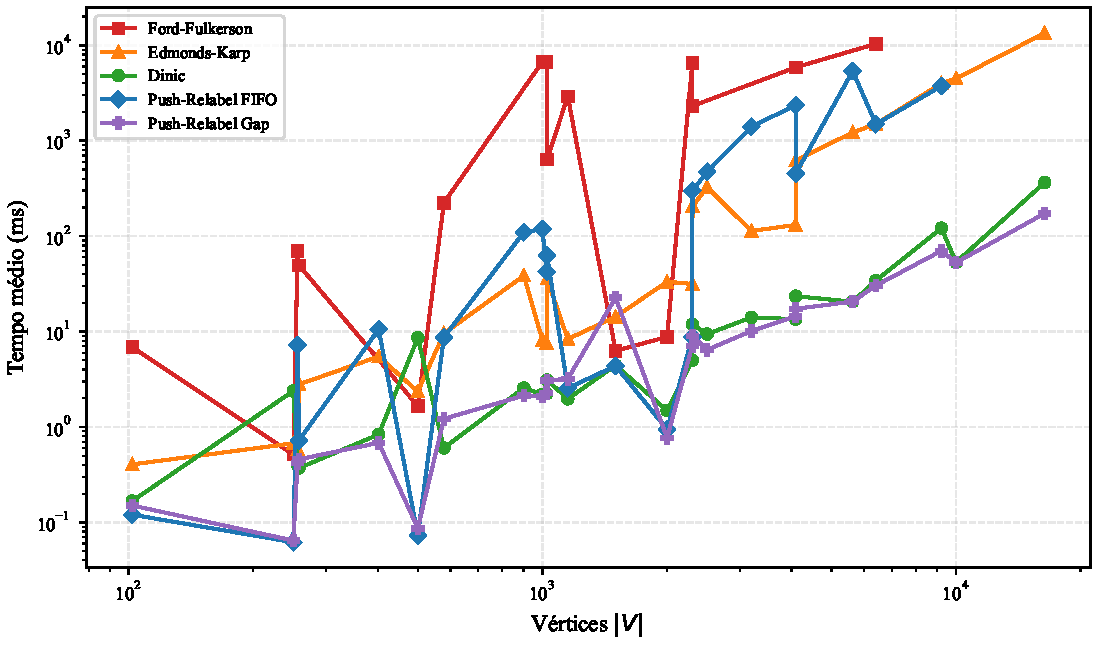
\includegraphics[width=0.92\textwidth]{figuras/scalability_maxflow}
    \caption{Escalabilidade dos algoritmos de fluxo máximo em função de $|V|$ (escala log-log).}
    \label{fig:scalability_maxflow_apendice}
\end{figure}

As curvas experimentais evidenciam a diferenciação entre as classes assintóticas:
\begin{itemize}[leftmargin=1.5em, itemsep=0.15em, topsep=0.2em, parsep=0em]
    \item \textbf{Ford-Fulkerson:} Apresenta forte sensibilidade às capacidades inteiras da rede. Nas instâncias lineares (\texttt{wash\_line\_50} e \texttt{wash\_line\_100}), onde $f^* > 7 \times 10^7$, o tempo de execução excede o limiar de 16 segundos (TLE), confirmando a dependência $O(|f^*| m)$;
    \item \textbf{Edmonds-Karp:} Mantém taxa de crescimento compatível com $O(n m^2)$, degradando em redes com grande diâmetro topológico em razão do custo de sucessivas buscas em largura ($O(m)$ por aumento);
    \item \textbf{Dinic e Push-Relabel com Heurística de Lacuna:} Apresentam as menores inclinações na escala log-log, indicando menor sensibilidade ao crescimento da rede e mantendo tempos inferiores a 70 ms mesmo em instâncias com mais de 10.000 vértices.
\end{itemize}

\subsection{Tabela Exaustiva e Escalabilidade: Fluxo de Custo Mínimo}

A Tabela~\ref{tab:benchmarks_mincost_exhaustive} reporta os dados experimentais completos dos quatro algoritmos de fluxo de custo mínimo na totalidade das 40 instâncias da família Netgen. O menor tempo por instância está destacado em \textbf{negrito}, e a indicação \textbf{TLE} denota interrupção por limite de 16 segundos.

\begingroup
\small
\setlength{\tabcolsep}{3.5pt}
\begin{longtable}{lrrrrrrrr}
\caption{Resultados experimentais exaustivos dos motores de fluxo de custo mínimo nas instâncias Netgen.}\label{tab:benchmarks_mincost_exhaustive}\\
\toprule
\textbf{Instância} & $|V|$ & $|A|$ & $f^*$ & $z^*$ & \textbf{CC} & \textbf{SSP-SPFA} & \textbf{SSP-Dijk} & \textbf{Simplex} \\
\midrule
\endfirsthead
\caption[]{Resultados experimentais exaustivos dos motores de fluxo de custo mínimo nas instâncias Netgen (continuação)}\\
\toprule
\textbf{Instância} & $|V|$ & $|A|$ & $f^*$ & $z^*$ & \textbf{CC} & \textbf{SSP-SPFA} & \textbf{SSP-Dijk} & \textbf{Simplex} \\
\midrule
\endhead
\bottomrule
\endfoot
\multicolumn{9}{l}{\textbf{Família DIMACS Netgen: Transbordo Inicial (01 a 10)}} \\
\midrule
\texttt{netgen\_01} & 202 & 1.508 & 100.000 & 196.587.626 & 350 & 11,0 & 15,1 & \textbf{5,07} \\
\texttt{netgen\_02} & 202 & 1.711 & 100.000 & 194.072.029 & 393 & 9,36 & 13,3 & \textbf{4,93} \\
\texttt{netgen\_03} & 202 & 2.200 & 100.000 & 159.442.947 & 620 & 16,4 & 16,9 & \textbf{6,44} \\
\texttt{netgen\_04} & 202 & 2.400 & 100.000 & 138.936.551 & 673 & 15,2 & 17,5 & \textbf{6,95} \\
\texttt{netgen\_05} & 202 & 3.100 & 100.000 & 102.950.805 & 1.071 & 22,3 & 23,7 & \textbf{9,07} \\
\texttt{netgen\_06} & 302 & 3.474 & 150.000 & 191.968.577 & 2.361 & 41,6 & 42,9 & \textbf{13,3} \\
\texttt{netgen\_07} & 302 & 4.819 & 150.000 & 172.742.047 & 3.565 & 53,1 & 54,5 & \textbf{19,6} \\
\texttt{netgen\_08} & 302 & 5.469 & 150.000 & 177.575.586 & 4.221 & 60,3 & 49,3 & \textbf{21,5} \\
\texttt{netgen\_09} & 302 & 6.375 & 150.000 & 144.994.180 & 5.976 & 61,1 & 57,0 & \textbf{23,2} \\
\texttt{netgen\_10} & 302 & 6.620 & 150.000 & 148.675.665 & 6.345 & 77,4 & 61,7 & \textbf{26,1} \\
\midrule
\multicolumn{9}{l}{\textbf{Família DIMACS Netgen: Transporte com Baixo Fluxo (11 a 15)}} \\
\midrule
\texttt{netgen\_11} & 402 & 1.900 & 200 & 473.532 & 94,8 & \textbf{7,79} & 16,0 & 11,2 \\
\texttt{netgen\_12} & 402 & 2.650 & 200 & 326.853 & 179 & \textbf{9,60} & 19,8 & 17,1 \\
\texttt{netgen\_13} & 402 & 3.400 & 200 & 258.242 & 262 & \textbf{12,8} & 20,3 & 21,6 \\
\texttt{netgen\_14} & 402 & 4.150 & 200 & 247.036 & 375 & \textbf{14,1} & 21,7 & 26,0 \\
\texttt{netgen\_15} & 402 & 4.900 & 200 & 212.597 & 446 & \textbf{15,7} & 23,3 & 30,2 \\
\midrule
\multicolumn{9}{l}{\textbf{Família DIMACS Netgen: Transporte com Alta Demanda (16 a 27)}} \\
\midrule
\texttt{netgen\_16} & 402 & 1.374 & 400.000 & 6.815.524.469 & 87,4 & 7,29 & 10,1 & \textbf{6,20} \\
\texttt{netgen\_17} & 402 & 2.511 & 400.000 & 2.646.770.386 & 283 & \textbf{7,22} & 10,2 & 9,61 \\
\texttt{netgen\_18} & 402 & 1.374 & 400.000 & 6.663.684.919 & 114 & 6,45 & 8,68 & \textbf{6,28} \\
\texttt{netgen\_19} & 402 & 2.511 & 400.000 & 2.618.979.806 & 282 & \textbf{7,74} & 10,7 & 8,41 \\
\texttt{netgen\_20} & 402 & 1.484 & 400.000 & 6.749.969.302 & 134 & 5,73 & 9,02 & \textbf{4,64} \\
\texttt{netgen\_21} & 402 & 2.904 & 400.000 & 2.631.027.973 & 304 & 7,88 & 10,8 & \textbf{7,34} \\
\texttt{netgen\_22} & 402 & 1.484 & 400.000 & 6.621.515.104 & 144 & \textbf{4,44} & 7,32 & 6,42 \\
\texttt{netgen\_23} & 402 & 2.904 & 400.000 & 2.630.071.408 & 361 & 8,83 & 10,0 & \textbf{6,35} \\
\texttt{netgen\_24} & 402 & 1.398 & 400.000 & 6.829.799.687 & 73,9 & \textbf{3,61} & 4,66 & 6,70 \\
\texttt{netgen\_25} & 402 & 2.692 & 400.000 & 6.396.423.129 & 190 & 11,3 & 10,5 & \textbf{8,76} \\
\texttt{netgen\_26} & 402 & 1.398 & 400.000 & 5.297.702.923 & 30,8 & \textbf{1,03} & 2,13 & 4,76 \\
\texttt{netgen\_27} & 402 & 2.692 & 400.000 & 4.863.992.745 & 118 & \textbf{5,14} & 5,82 & 6,78 \\
\midrule
\multicolumn{9}{l}{\textbf{Família DIMACS Netgen: Grande Escala (28 a 35)}} \\
\midrule
\texttt{netgen\_28} & 1.002 & 3.000 & 1.000.000 & 11.599.233.408 & 1.420 & \textbf{22,2} & 28,4 & 37,4 \\
\texttt{netgen\_29} & 1.002 & 3.500 & 1.000.000 & 11.700.773.092 & 1.380 & \textbf{31,1} & 35,5 & 39,8 \\
\texttt{netgen\_30} & 1.002 & 4.500 & 1.000.000 & 8.782.721.260 & 2.479 & 40,7 & \textbf{37,8} & 56,4 \\
\texttt{netgen\_31} & 1.002 & 4.900 & 1.000.000 & 8.577.913.734 & 2.145 & \textbf{38,8} & 40,4 & 53,5 \\
\texttt{netgen\_32} & 1.502 & 4.492 & 1.500.000 & 17.996.365.110 & 5.796 & 66,8 & \textbf{65,5} & 107 \\
\texttt{netgen\_33} & 1.502 & 4.535 & 1.500.000 & 18.424.893.900 & 4.926 & 82,7 & \textbf{68,8} & 111 \\
\texttt{netgen\_34} & 1.502 & 5.257 & 1.500.000 & 14.596.094.907 & 6.044 & 70,6 & \textbf{69,3} & 105 \\
\texttt{netgen\_35} & 1.502 & 5.880 & 1.500.000 & 14.350.903.861 & 8.176 & 113 & \textbf{90,9} & 123 \\
\midrule
\multicolumn{9}{l}{\textbf{Família DIMACS Netgen: Escala Máxima (36 a 40)}} \\
\midrule
\texttt{netgen\_36} & 8.002 & 16.200 & 4.000.000 & 87.957.673.940 & TLE & 5.172 & \textbf{3.497} & 4.047 \\
\texttt{netgen\_37} & 5.002 & 23.950 & 4.000.000 & 35.607.266.430 & TLE & 4.817 & \textbf{3.064} & 4.091 \\
\texttt{netgen\_38} & 3.002 & 35.625 & 2.000.000 & 7.265.734.372 & TLE & 3.480 & \textbf{1.978} & 2.107 \\
\texttt{netgen\_39} & 5.002 & 15.880 & 4.000.000 & 48.660.418.428 & TLE & 2.898 & \textbf{2.089} & 2.862 \\
\texttt{netgen\_40} & 3.002 & 23.400 & 2.000.000 & 11.068.572.024 & TLE & 1.440 & \textbf{961} & 1.543 \\
\end{longtable}
\endgroup


A Figura~\ref{fig:scalability_mincost_apendice} apresenta as curvas de tempo em função de $|V|$ para os algoritmos de custo mínimo na família Netgen.

\begin{figure}[!ht]
    \centering
    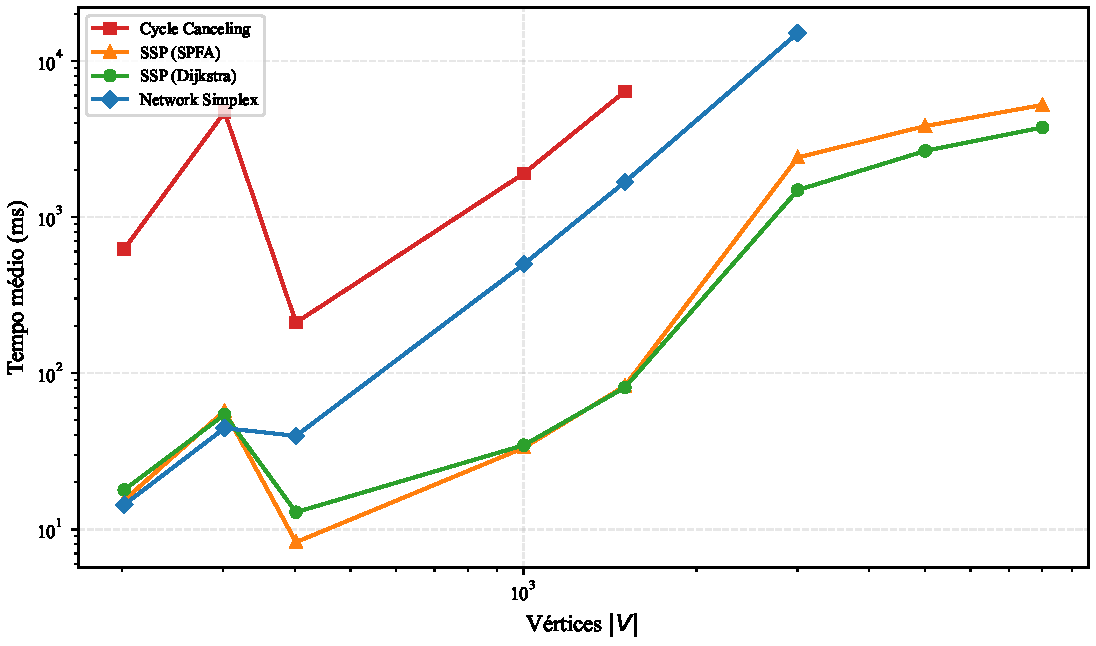
\includegraphics[width=0.92\textwidth]{figuras/scalability_mincost}
    \caption{Escalabilidade dos algoritmos de fluxo de custo mínimo em função de $|V|$ (escala log-log).}
    \label{fig:scalability_mincost_apendice}
\end{figure}

Observa-se que a inclinação da curva do \textit{Cycle Canceling} é expressivamente superior à dos métodos \textit{Successive Shortest Path} e \textit{Network Simplex}, refletindo o custo de detecção global de ciclos negativos a cada iteração.
